\documentclass[12pt]{article}
\usepackage[brazilian]{babel}
\usepackage[utf8]{inputenc}
\usepackage{setspace}
\usepackage{boxedminipage}
\usepackage{amsmath}
\usepackage{latexsym}
\usepackage{multirow}
\usepackage[pdftex]{graphicx}
\usepackage{float}
\usepackage{url}
\usepackage{tikz}
\usepackage{blkarray}

\renewcommand{\familydefault}{\sfdefault}
\newcommand{\question}[2] {\vspace{0.3in}\noindent{\subsection*{Exercício #1. #2} \vspace{0.15in}}}
\renewcommand{\part}[1] {{\vspace{0.15in}\noindent\textbf (#1)} \vspace{0.10in}}
\newcommand{\answer}[1]{{\fontfamily{\rmdefault}\selectfont \textbf{R:} #1}}
\newcommand{\overbar}[1]{\mkern 2mu\overline{\mkern-2mu#1\mkern-2mu}\mkern 2mu}

%\setlength{\parskip}{0.1cm}
\setlength{\paperheight}{29.7cm}
\setlength{\textheight}{23.0cm}
\setlength{\textwidth}{16.5cm}
\setlength{\oddsidemargin}{0.0cm}
\setlength{\topmargin}{-1.0cm}
\pagestyle{empty}


\begin{document}
\title{Exercício - Modelagem de Bancos de Dados NoSQL}
\author{\large Gustavo Estrela de Matos}
\date{\today}
\maketitle

Considerando a quantidade e complexidade do relacionamentos entre os
objetos de interesse do problema, consideramos que usar uma modelagem de
banco de dados de grafos seria adequada. Criamos portanto o modelo 
descrito abaixo.

As entidades que identificamos são apresentadas no diagrama abaixo. Em
seguida, mostramos uma breve descrição das entidades, assim como uma
descrição de alguns atributos novos, que não foram mencionados no 
enunciado.
\vspace{1em}

\begin{center}
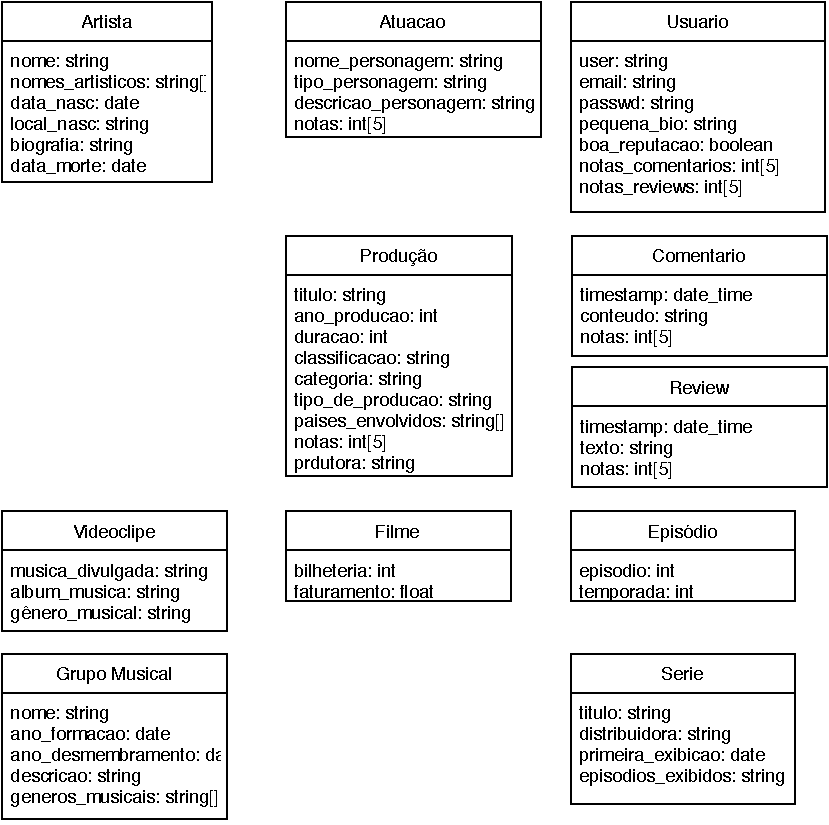
\includegraphics[width=.8\linewidth]{entities_bdgrafos.pdf}
\end{center}

\begin{itemize}
    \item{\bf Artista}: representa um artista, que podem ser diretor,
        ator ou músico. O atributo {\ttfamily nomes\_artisticos} 
        armazena todos os nomes artísticos deste mesmo artista.
    \item{\bf Grupo Musical}: representa um grupo musical.
    \item{\bf Produção}: representa alguma produção em formato de vídeo.
        O atributo {\ttfamily tipo\_de\_producao} indica se a produção é
        um videoclipe, um filme ou episódio de uma série. Além disso, o
        array {\ttfamily notas} armazena a quantidade de notas 
        (de 1 a 5) que foram dadas por usuários para a produção.
    \item{\bf Videoclipe}: representa uma produção que é um videoclipe. 
        Cada videoclipe apresenta uma música, que tem um gênero musical 
        e possivelmente um álbum no qual a música foi lançada.
    \item{\bf Filme}: representa uma produção que é um filme.
    \item{\bf Episódio}: representa um episódio de uma série.
    \item{\bf Serie}: armazena dados sobre uma série. O atributo 
        {\ttfamily temporada} indica a qual temporada o episodio 
        pertence; caso não existam diferentes temporadas, o valor deste
        atributo é nulo.
    \item{\bf Atuação}: representa a atuação de um artista em alguma 
        produção. Assim como em Produção, o array {\ttfamily notas} 
        armazena as notas (de 1 a 5) dadas para a atuação.
    \item{\bf Usuário}: representa um usuário da aplicação. O atributo
        {\ttfamily good\_reputation} é uma flag que indica se o usuário
        tem boa reputação ou não. Os atributos 
        {\ttfamily notas\_comentarios} e {\ttfamily notas\_reviews}
        armazenam as notas (de 1 a 5) que os comentários e reviews deste 
        usuário receberam.
    \item{\bf Comentário}: armazena comentários feitos a produções
        ou a atuações. O atributo {\ttfamily notas} armazena as notas
        que este comentário recebeu de usuários.
    \item{\bf Review}: armazena reviews feitas a produções. O atributo
        {\ttfamily notas} armazena as notas que este review recebeu de
        usuários.
\end{itemize}


Abaixo, apresentamos os relacionamentos entre estas entidades, em um 
diagrama do modelo de bancos de dados de grafos para a aplicação.

\begin{center}
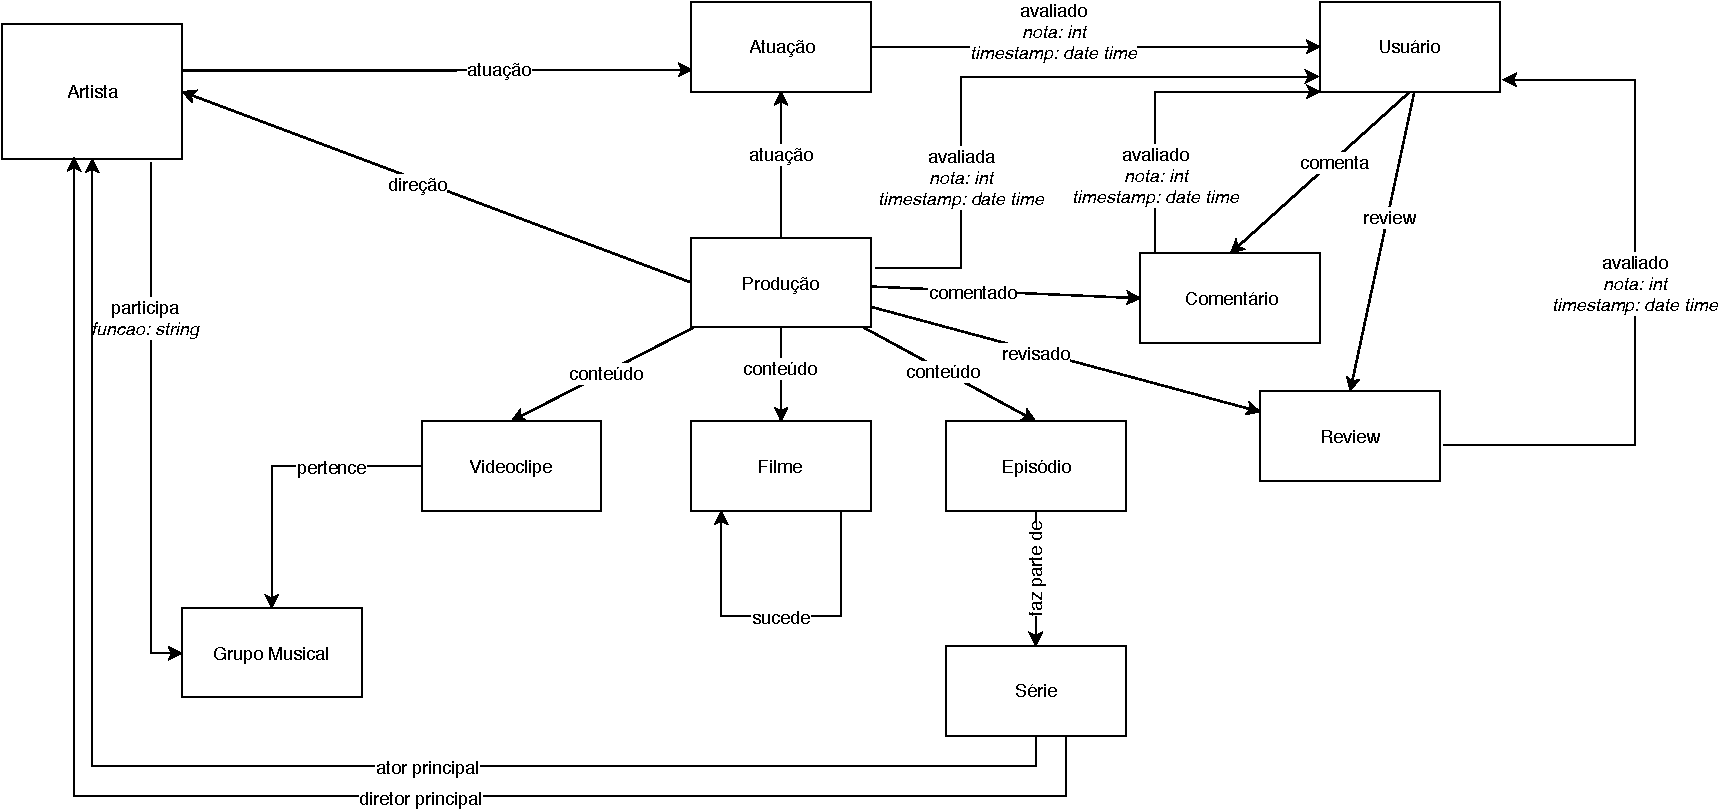
\includegraphics[width=\linewidth]{Diagrama_bdgrafos1.pdf}
\end{center}

Vamos discutir o desempenho deste modelo quando consideramos as
principais consultas da aplicação.

\begin{enumerate}
    \item{\bf Recuperar dados dos vídeos dirigidos por um dado diretor}
        
        Basta percorrer todos os arcos "direção" que chegam no nó do
        diretor dado. Podemos considerar que esta operação é realizada
        com bom desempenho, pois a identificação do nó do diretor deve
        ser rápida (pois os nós são indexados), e descobrir os vídeos
        que ele dirigiu depende apenas de percorrer os arcos "direção"
        que partem do nó.

    \item{\bf Recuperar dados dos videoclipes de um dado grupo musical}

        Basta percorrer os arcos "pertence" que chegam no nó do grupo
        musical. Novamente, podemos considerar bom o desempenho desta
        operação, pois ela depende apenas da identificação do nó do
        grupo musical e do percorrimento de arcos que chegam neste nó.

    \item{\bf Obter os nomes de atores que já aturam como diretor (ou 
        vice-versa)}

        Para realizar esta operação é necessário percorrer todos os nós 
        de artistas e descobrir os nós que possuem arcos "direção" 
        chegando e arcos "atuação" saindo. Esta operação deve ter bom
        desempenho, desde que o número de artistas não seja muito 
        grande.

    \item{\bf Obter dados dos filmes que são comédias musicais}
        
        Cada nó do tipo filme está ligado a um (e apenas um) nó 
        Produção. Portanto, para realizar esta consulta, é necessário 
        percorrer todos os nós do tipo filme, e selecionar aqueles que
        estão ligados a um nó Produção que tenha no atributo 
        {\ttfamily categoria} o valor "comédia musical". Novamente,
        o bom desempenho desta consulta depende que a quantidade de 
        filmes registrados no banco de dados.

    \item{\bf Obter todas as sequências (diretas e indiretas) de um dado 
        filme}
        
        Para descobrir a sequência direta de um filme, basta identificar
        a ponta final do arco "sucede" que sai do filme de interesse.
        Assim, para descobrir todos os sucessores de um filme, basta 
        fazer este procedimento recursivamente até o último filme. De 
        maneira similar, podemos usar a ponta inicial do arco "sucede" 
        que chega a um filme para identificar seu antecessor direto.  
        Portanto, com estes arcos, é possível obter todos os filmes de 
        uma série de filmes. A execução desta tarefa deve ser eficiente
        porque não precisa percorrer uma grande quantidade de nós ou 
        arcos.

    \item{\bf Obter os nomes de atores que atuaram em uma dada série}
        
        Para responder esta consulta, precisamos primeiro descobrir 
        todos os nós Episódio que estão conectados a série de interesse
        pelo arco "faz parte de". Em seguida, é necessário verificar o 
        nó Produção correspondente a cada nó Episódio da série, e 
        também percorrer todos os nós Atuação ligados a estes nós 
        Produção, para enfim descobrir o nome dos artistas pelo arco
        "atuação" ligado aos nós Atuação. Esta consulta pode ter um
        desempenho ruim, pois é necessário percorrer todos os nós 
        Episódios, mesmo que um ator tenha atuado em diversos episódios
        desta série. Para esta consulta ser executada com melhor 
        desempenho, podemos adicionar um arco redundante "atua na serie" 
        que liga Artista e Série sempre que um artista atua em um 
        episódio de uma série.

    \item{\bf Obter a nota média de uma produção ou de uma atuação}

        Para obter a nota média de uma atuação, precisamos apenas 
        acessar o atributo {\ttfamily notas}. Sempre que um usuário
        dá uma nota para a atuação, este vetor é atualizado somando-se
        um na posição referente a nota. Note que este atributo é 
        redundante, pois esta informação também está presente no arco
        "avaliado" que conecta um nó Atuação com um nó Usuário; 
        entretanto, manter essa informação no nó Atuação facilita o 
        cálculo da nota média da atuação.

    \item{\bf Obter a lista de produções mais bem avaliadas na última 
        semana}
        \label{consulta8}
        
        Para se responder esta consulta é necessário percorrer todos os
        arcos "avaliada" entre Produção e Usuário, considerando apenas
        aqueles que foram criados na última semana. Esta consulta 
        provavelmente terá desempenho ruim com o aumento de avaliações
        armazenadas, considerando que ela precisa percorrer todos os 
        arcos de avaliação do sistema.

    \item{\bf Obter os identificadores dos usuários que fizeram os 
        comentários mais bem avaliados no último mês}
        \label{consulta9}

        Para se responder esta consulta é necessário percorrer todos os
        arcos "avaliado" entre Comentário e Usuário, considerando apenas
        aqueles que foram criados no último mês. Pelo mesmo motivo da 
        última consulta, esta consulta também não terá bom desempenho
        quando o número de avaliações a comentários for grande.
\end{enumerate}


Identificamos então que este modelo possibilita a realização das 
consultas com bom desempenho, exceto pelas consultas \ref{consulta8} e
\ref{consulta9}. Ambas consultas estão relacionadas a avaliações feitas
por usuários, a comentários de outros usuários ou a produções. Vamos
então, utilizar outro banco de dados para armazenar apenas as avaliações
a comentários, produções, reviews e atuações.

Como estamos interessados em obter avaliações recentes, considerando 
últimos meses ou semanas, vamos utilizar um modelo baseado em agregados 
que nos permite selecionar os últimos meses ou semanas de avaliações. 
Escolhemos então utilizar o modelo chave-valor, considerando nossa chave
como o time-stamp (como um inteiro) da avaliação. O diagrama com o 
agregado é representado abaixo.

\begin{center}
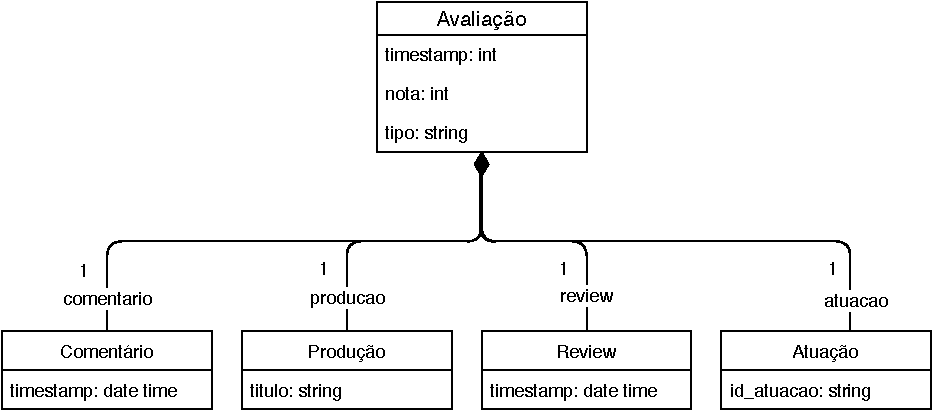
\includegraphics[width=.8\linewidth]{agregados_avaliacao.pdf}
\end{center}

Este agregado é composto pelos atributos da avaliação e por mais um
atributo chamado {\ttfamily tipo} que determina o tipo de avaliação: de 
comentário, de produção, de review ou de atuação. Além disso, o agregado
também contém um (e apenas um) componente que pode ser do tipo 
Comentário, Produção, Review ou Atuação (entidades deste banco de 
avaliações). Cada uma destas entidades contém um valor que identifica o 
seu nó correspondente no banco de dados de grafos.

Para responder a consulta~\ref{consulta8}, podemos selecionar
todas as avaliações feitas para produções na última semana e calcular
aquela que foi melhor avaliada com um agrupamento por produção. De 
maneira similar, podemos responder a consulta~\ref{consulta9} após
selecionar todas avaliações a comentários feitas no último mês e 
calcular um agrupamento destas avaliações por usuário.

Agora, basta adaptar o banco de dados de grafos, que não precisa mais
dos relacionamentos de avaliação, pois os mesmos serão armazenados no
banco de dados chave-valor. Além disso, criamos um novo atributo em
Atuação, que nos permite identificar um nó de maneira unívoca. As 
entidades do banco de dados de grafos e o diagrama deste banco são 
apresentados abaixo.

\begin{center}
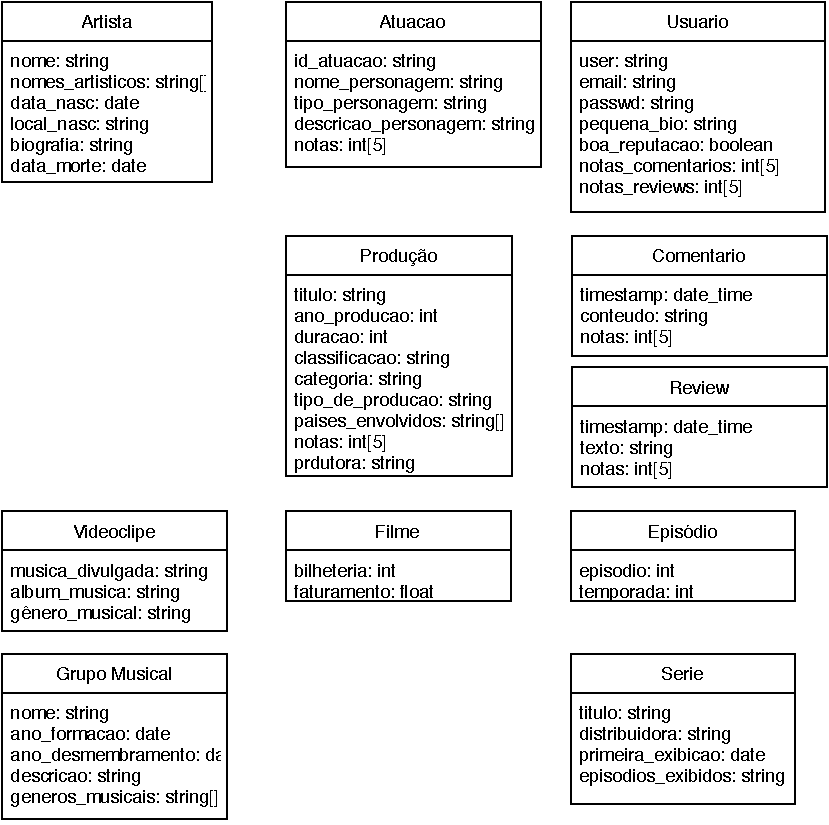
\includegraphics[width=.8\linewidth]{entities_bdgrafos2.pdf}
\vspace{2em}
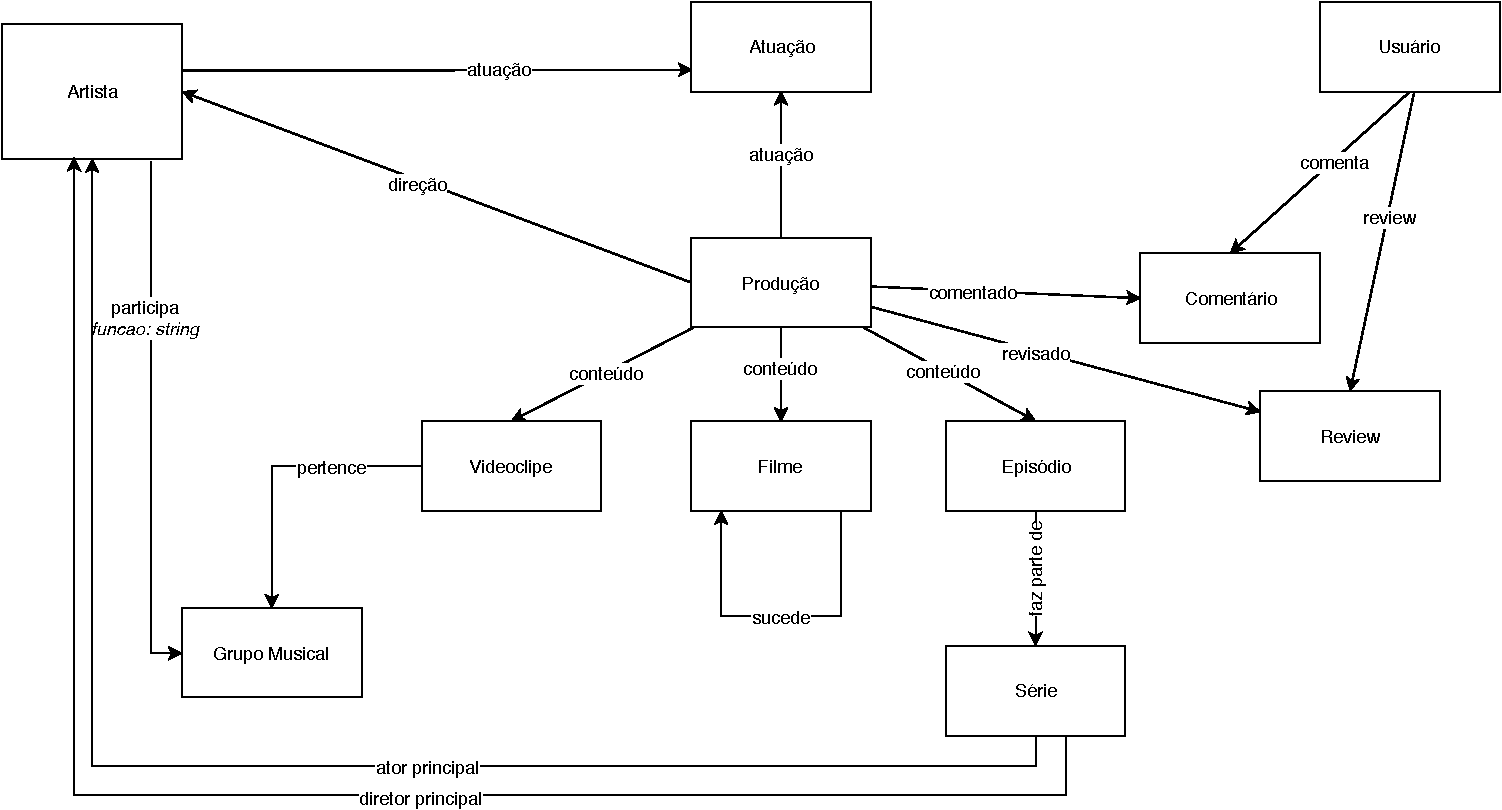
\includegraphics[width=\linewidth]{Diagrama_bdgrafos2.pdf}
\end{center}

\end{document}
